% Beginning code for all standard physics latex documents

%Created on: May 8, 2014    Edited by: Wesley Kyle
%Edited on:	May 12, 2016	Edited by: P. Gimby - cleaned up the code to remove unneeded packages
%Edited on:	May 13, 2016	Edited by: P. Gimby - collected a few more packages used in 325.
%Edited on:	May 16, 2016	Edited by: P. Gimby - fixed page numbering error.
%Edited on: May 20, 2016	Edited by: Alex Shook - Added packages for 497

\documentclass[justified]{tufte-book}
\usepackage{graphicx} % allow embedded images
\setkeys{Gin}{width=\linewidth,totalheight=\textheight,keepaspectratio}
\usepackage{amsmath}  % extended mathematics
\usepackage{bm}  % bold font in math mode
\usepackage{longtable} %lets long tables flow into multiple pages instead of running off the page or having to break tables up manually
\usepackage{booktabs} % book-quality tables
\usepackage{units}    % non-stacked fractions and better unit spacing
\usepackage{multicol} % multiple column layout facilities
\usepackage{tikz} %for drawing nice pictures
\usepackage{indentfirst} % makes first line of each new section be indented
\usepackage{enumitem} % extended options for the enumerate environment
\usepackage{soul} % gives more typestting options like spacing, underline, and strike-through
\usepackage{marvosym} %extra symbols package
\usepackage{multirow} % for special table controls
\usepackage[singlelinecheck=false]{caption} % allow captions w/o figure number
\captionsetup{compatibility=false} % corrects in issue with the caption package
\usepackage{float} % allows for contorl over position of figures and tables
\allowdisplaybreaks % allows equations to span two pages if needed
\usepackage{mathrsfs} % fancy math symbols
\usepackage{multirow} % for special table controls
\usetikzlibrary{arrows,shapes,snakes,calc,patterns,3d} % addon to tikz
\usetikzlibrary{circuits.ee.IEC} % addon to tikz
\usepackage{pgfplots} % package for making plots of functions
\usepackage{gensymb} % symbols i,e. degrees
\usetikzlibrary{decorations.pathmorphing} % to draw the springs
\tikzset{circuit declare symbol = ac source}
\tikzset{set ac source graphic = ac source IEC graphic}
\usepackage{changepage} % allows for full page environment
\usepackage{comment} % allows comment tags for large sections

% define new page style that puts page numbers in the middle
%\begin{comment}
\fancypagestyle{custom}{
\fancyhf{} % clear all header and footer fields
\fancyheadoffset{0pt}
\fancyfootoffset{0pt}
\fancyfoot[C]{\thepage}
\renewcommand{\headrulewidth}{0pt}
\renewcommand{\footrulewidth}{0pt}}
\pagestyle{custom}
%\end{comment}

%below creates a new circuit symbol for AC sources
\tikzset{
         ac source IEC graphic/.style=
          {
           transform shape,
           circuit symbol lines,
           circuit symbol size = width 3 height 3,
           shape=generic circle IEC,
           /pgf/generic circle IEC/before background=
            {
             \pgftransformresetnontranslations
             \pgfpathmoveto{\pgfpoint{-0.8\tikzcircuitssizeunit}{0\tikzcircuitssizeunit}}
             \pgfpathsine{\pgfpoint{0.4\tikzcircuitssizeunit}{0.4\tikzcircuitssizeunit}}
             \pgfpathcosine{\pgfpoint{0.4\tikzcircuitssizeunit}{-0.4\tikzcircuitssizeunit}}
             \pgfpathsine{\pgfpoint{0.4\tikzcircuitssizeunit}{-0.4\tikzcircuitssizeunit}}
             \pgfpathcosine{\pgfpoint{0.4\tikzcircuitssizeunit}{0.4\tikzcircuitssizeunit}}
             \pgfusepathqstroke
            }
          }
        }
% end of circuit symbol
%\begin{document}
%%%end individual beginning code/,$d


%  \begin{titlepage}
%    \vspace*{\fill}
%    \begin{center}
%      \huge{{\bf TITLE1}}\\[0.4cm]
%      \huge{TITLE2}\\[0.4cm]
%      \LARGE{Laboratory Manual}\\[0.4cm]
%      \large{SEASON YEAR}
%    \end{center}
%    \vspace*{\fill}
%  \end{titlepage}
%\maketitle

%\begin{spacing}{0.5}
%\tableofcontents
%\end{spacing}

%NEW PHYS 497 PACKAGES AND COMMANDS

%Subcaption package: Allows subfigures to be placed side by side, and labeled with individual captions (Added June 1, 2016)
\usepackage{subcaption}

%Array package: Allows for addiation specifications in arrays (Added May 6, 2016)
\usepackage{array}

%newcolumntype: Allows one to specify a fixed column width (Added May 6, 2016)
\newcolumntype{L}[1]{>{\raggedright\let\newline\\\arraybackslash\hspace{0pt}}m{#1}}
\newcolumntype{C}[1]{>{\centering\let\newline\\\arraybackslash\hspace{0pt}}m{#1}}
\newcolumntype{R}[1]{>{\raggedleft\let\newline\\\arraybackslash\hspace{0pt}}m{#1}}

%circuits.logic.US, circuits.logic.IEC: For drawing logic gates in Tikz (Added May 6, 2016) 
\usetikzlibrary{circuits.logic.US,circuits.logic.IEC}

\newcommand{\PGT}{ %PGT: positive going transition
\begin{tikzpicture}
\draw[-angle 60] (0,0) -- (0,5pt);
\draw (0,5pt) -- (0,6pt) -- (5pt,6pt);
\draw (-5pt,0) -- (0,0);
\end{tikzpicture}
}





%TEST
\usepackage{geometry}
\pagestyle{fancy}

%\usepackage[caption=false]{subfig}

%\makeatletter
%\renewenvironment{figure}[1][htbp]{%
%  \@tufte@orig@float{figure}[#1]%
%}{%
%  \@tufte@orig@endfloat
%}

%\renewenvironment{table}[1][htbp]{%
%  \@tufte@orig@float{table}[#1]%
%}{%
%  \@tufte@orig@endfloat
%}
%\makeatother

% use instead of subfigure
\makeatletter
\newenvironment{multifigure}[1][htbp]{%
  \@tufte@orig@float{figure}[#1]%
}{%
  \@tufte@orig@endfloat
}
\makeatother

\makeatletter
\newenvironment{mainfigure}[1][htbp]{%
\@tufte@orig@float{figure}[#1]
\begin{adjustwidth}{}{-153pt}}
{\end{adjustwidth}\@tufte@orig@endfloat}%
\makeatother

\makeatletter
\newenvironment{maintable}[1][htbp]{%
\@tufte@orig@float{table}[#1]
\begin{adjustwidth}{}{-153pt}}
{\end{adjustwidth}\@tufte@orig@endfloat}%
\makeatother

%%%% Labatorial Cross-over labs need this code. This should be temporary PG Dec 7, 2016

\newcounter{questioncounter}
\setcounter{questioncounter}{0}
\newcounter{checkpointcounter}
\setcounter{checkpointcounter}{0}
\newcounter{figurecounter}
\setcounter{figurecounter}{0}
%%%%%%%%%%%%%%%%%%%%%%%%%%%%%%%%%%%%%%%%%%%%%%%%%%%%%%%

\newcommand{\checkpoint}{
 \fbox{\begin{minipage}{0.2\textwidth}
 %\includegraphics[width=0.5\textwidth]{stop}
 \end{minipage}
 \begin{minipage}{1.0\textwidth}
 {\bf CHECKPOINT \addtocounter{checkpointcounter}{1} \arabic{checkpointcounter}: Before moving on to the next part, have your TA check the results you obtained so far.}
 \end{minipage}}}

%%% end labatorial cross-over code.

% New environment for placing figure captions under the figure
%\makeatletter
%\newenvironment{mainfigure}{\textwidth}[1][htbp]{%
%\@tufte@orig@float{figure}[#1]%
%}{%
%\@tufte@orig@endfloat
%}
%\makeatother

\begin{document}
%%%%%%%%%%%%%%%%%%%%%%%%%%%%%%%%%%%%%%%%%%%%%
%
% 0101 PHYS397FA2017
%
%%%%%%%%%%%%%%%%%%%%%%%%%%%%%%%%%%%%%%%%%%%%%


\setcounter{chapter}{2}
\setcounter{equation}{0}
\setcounter{table}{0}
\setcounter{figure}{0}
\chapter{Voltage Dividers and Voltage Sources}

\section{Equipment}

% first column
\begin{minipage}{0.5\textwidth}
\begin{itemize}[noitemsep]
\item Anatek power supply
\item Philips multimeter
\item Sanwa 501 analog multimeter
\item Set of 3 resistors
\end{itemize}
\end{minipage}
%second column
\begin{minipage}{0.5\textwidth}
\begin{itemize}[noitemsep]
\item Set of 2 resistors
\item Eico 1171 decade resistor box
\item 25 $\Omega$ Potentiometer
\item Black box voltage divider
\item Set of connecting leads (3)
\end{itemize}
\end{minipage}

\begin{marginfigure}%[-2in]
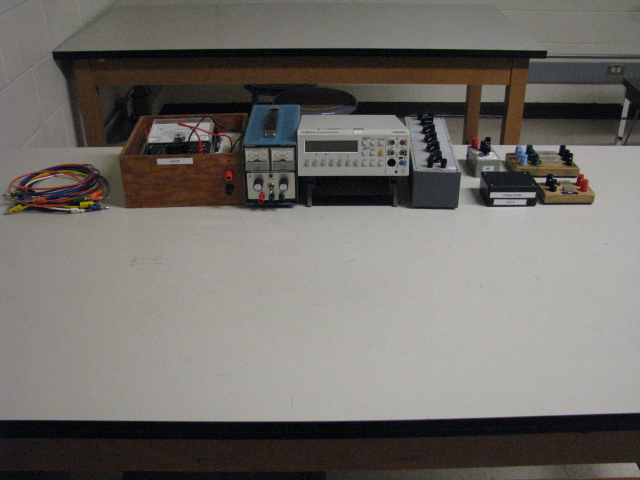
\includegraphics{/usr/local/master/labs/physics397-FA2017/0101-PHYS397FA2017/Voltage-Dividers-and-Voltage-Sources-Setup.jpg}
\caption{Equipment Setup}
\label{pic:vdSetup}
\end{marginfigure}

\section{Preparation}
% copy and paste the section under preparation (or similar section)
Review the basic ideas of circuit analysis including Ohm's law and Kirchhoff's laws.

\section{Goals of the Experiment}
% copy and paste the section under goals of the experiment (or similar section)
\begin{itemize}
    \item To investigate voltage dividers and their uses.
    \item To understand the concepts of internal resistance and Th\'{e}venin equivalence.
    \item To get experience with potentiometers, power supplies, and voltmeters, and gain a better understanding of how they work. 
    \item To observe the effects of circuit loading and how this affects measurements.
\end{itemize}
%To investigate voltage dividers and their uses. To understand the concepts of internal resistance and Th�venin equivalence. To
%get experience with potentiometers, power supplies, and voltmeters, and gain a better understanding of how they work. To 
%observe the effects of circuit loading and how this affects measurements.

\section{Theory}

\begin{marginfigure}
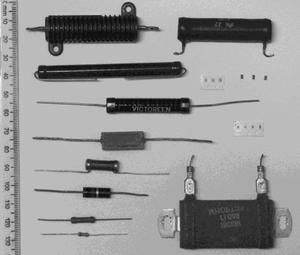
\includegraphics{/usr/local/master/labs/physics397-FA2017/0101-PHYS397FA2017/Voltage-Dividers-and-Voltage-Sources-Resistors.jpg}
\caption{Examples of resistors of different shapes and sizes}
\label{pic:vdResistors}
\end{marginfigure}

The use of electric circuits today is a large part of everyday life. The radio, television, telephone and computer are all examples of devices that use electric circuits. In almost all circuits \textbf{resistors} are among the most common components. Figure \ref{pic:vdResistors} shows some of the many different kinds of resistors. The different shapes and sizes play a role in their behavior and application. Resistors are used to control the current and voltage in a circuit. They were extensively studied by physicists due to this property. Whether it is a complex circuit, such as the ones found in a computer, or one as simple as a battery connected to a light bulb, there are fundamental rules that all resistor circuits follow.			

Georg Ohm (1789-1854) contributed largely to what is now known about resistors. He speculated how current might work and formulated the law governing resistors that now bears his name. Later, Gustav Kirchhoff (1824-1887) made further contributions to the understanding of electric circuits. He extended Ohm's work describing what are now call \textbf{Kirchhoff's Laws}, which explained how current and voltage in electric circuits are related. In 1883 L\'{e}on Th\'{e}venin (1857-1926), a French telegraph engineer, described what he thought to be a new theory of equivalent circuits. He showed that any resistor circuit could be simplified to make analysis easier. Coincidentally, the concept of equivalency in circuits had already been proposed almost 30 years earlier by the physicist Herman von Helmholtz (1821-1894). Th\'{e}venin was unaware of Helmholtz's work and both theories met with resistance during their time. It was due to Th\'{e}venin's engineering approach, and the growth of electrical engineering in the coming years, that his result is now called \textbf{Th\'{e}venin's Theorem}.

\begin{marginfigure}
%\usetikzlibrary{arrows,snakes,shapes,calc,patterns}
%\usetikzlibrary{circuits.ee.IEC}
      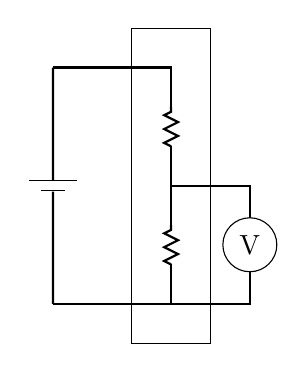
\begin{tikzpicture}[circuit ee IEC]
      \draw[thick] (0,3) to [battery] (0,0); % battery
      \draw[thick] (0,0) -- (1.5,0) -- (1.5,0.5)(1.5,1) -- (1.5,2)(1.5,2.5) -- (1.5,3) -- (0,3);  %wiring
      \draw[snake=zigzag,segment length=5,thick] (1.5,2) -- (1.5,2.5); % upper resistor
      \draw[snake=zigzag,segment length=5,thick] (1.5,0.5) -- (1.5,1); % lower resistor
      \draw[thick] (1.5,1.5) -- (2.5,1.5) -- (2.5,0) -- (1.5,0); % voltmeter wires
      \node[black,fill=white,draw=black,shape=circle,scale=1] at (2.5,0.75) {V}; % voltmeter
      \draw (1,-0.5) rectangle (2,3.5); % voltage divider box
\end{tikzpicture}
\caption{Basic voltage divider with power supply}
\label{fig:vdBasicVD}
\end{marginfigure}

Many combinations of resistors exist in circuitry, but the \textbf{voltage divider} is one combination that is seen everywhere. The circuit in Figure \ref{fig:vdBasicVD} contains a voltage source of some kind, connected in series loop with two resistors. A voltmeter is in parallel with one of the resistors to measure the voltage across it. Each resistor in the loop drops a portion of the voltage. This resistor combination, which accomplishes the splitting of voltages, is called a voltage divider. It can be used to control the voltages coming out of, or going into, a particular system, or even be used as a tool for analysis of circuits.

\begin{marginfigure}
  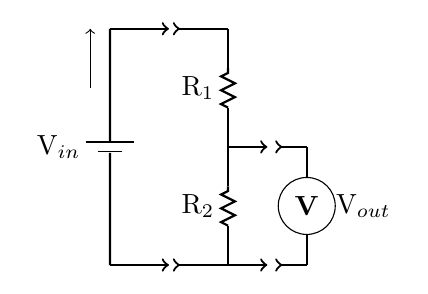
\begin{tikzpicture}[circuit ee IEC]
      \draw[thick] (0,3) to [battery] (0,0); % battery
      \node at (-0.65,1.5) {V$_{in}$}; % Vin label
%      \node at (-0.45,1.4) {\small{in}}; % Vin label
      \draw[thick,->] (0,0) -- (0.75,0); % Wiring 
      \draw[thick,>->] (0.8,0) -- (2,0); % Wiring
      \draw[thick,->] (0,3) -- (0.75,3); % Wiring
      \draw[thick,>-] (0.8,3) -- (1.5,3); % Wiring
      \draw[thick](1.5,0) -- (1.5,0.5)(1.5,1) -- (1.5,2)(1.5,2.5) -- (1.5,3); % Wiring
      \draw[snake=zigzag,segment length=5,thick] (1.5,2) -- (1.5,2.5); % upper resistor
      \node[left] at (1.45,2.25){R$_{1}$}; % R1 label
      \draw[snake=zigzag,segment length=5,thick] (1.5,0.5) -- (1.5,1); % lower resistor
      \node[left] at (1.45,0.75){R$_{2}$}; % R2 label
      \draw[thick] (2.5,1.5) -- (2.5,0); % voltmeter wires
      \draw[thick,->] (1.5,1.5) -- (2,1.5); % Wiring
      \draw[thick,>-] (2.1,1.5) -- (2.5,1.5); % Wiring
      \draw[thick,>-] (2.1,0) -- (2.5,0); % Wiring
      \node[black,fill=white,draw=black,shape=circle,scale=1] at (2.5,0.75) {\textbf{V}}; % voltmeter   
      \node[right] at (2.75,0.75) {V$_{out}$}; % Vout label
      \draw[->](-0.25,2.25) -- (-0.25,3); % current arrow
    \end{tikzpicture}
    \caption{Connections for the voltage divider to voltage source and voltmeter}
    \label{fig:vdVoltDivConnect}
\end{marginfigure}

In Figure \ref{fig:vdVoltDivConnect} the connections of the voltage divider to the voltage source and voltmeter are explicitly shown. The voltage source is supplying a voltage with magnitude V$_{in}$ into the voltage divider and the voltmeter reads V$_{out}$ across R$_{2}$. This suggests the voltage divider can be generalized further by extracting it from the circuit. Figure \ref{fig:vdVoltDivIsolated} shows only the voltage divider. The input voltage, V$_{in}$, can be generalized to be any source of voltage such as a battery, power supply or another device. The output voltage, V$_{out}$, is what would be applied to any device or system connected to these two terminals.


\begin{marginfigure}
  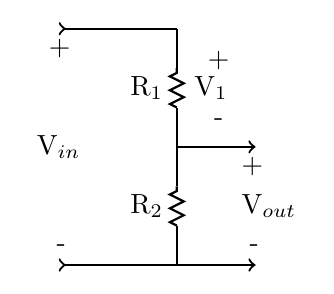
\begin{tikzpicture}
      \node at (0,1.5) {V$_{in}$}; % Vin label
      \node[right] at (-0.25,2.75) {+}; % Vin + label
      \node[right] at (-0.15,0.25) {-}; % Vin - label
      \draw[thick,>->] (0,0) -- (2.5,0); % Wiring 
      \draw[thick,>-] (0,3) -- (1.5,3); % Wiring
      \draw[thick](1.5,0) -- (1.5,0.5)(1.5,1) -- (1.5,2)(1.5,2.5) -- (1.5,3); % Wiring
      \draw[snake=zigzag,segment length=5,thick] (1.5,2) -- (1.5,2.5); % upper resistor
      \node[left] at (1.45,2.25){R$_{1}$}; % R1 label
      \draw[snake=zigzag,segment length=5,thick] (1.5,0.5) -- (1.5,1); % lower resistor
      \node[left] at (1.45,0.75){R$_{2}$}; % R2 label
      \draw[thick,->] (1.5,1.5) -- (2.5,1.5); % Wiring
      \node[right] at (2.2,0.75) {V$_{out}$}; % Vout label
      \node[right] at (2.2,1.25) {+}; % Vout + label
      \node[right] at (2.3,0.25) {-}; % Vout - label
      \node[right] at (1.6,2.25) {V$_{1}$}; % V1 label
      \node[right] at (1.77,2.6) {+}; % V1 + label
      \node[right] at (1.85,1.85) {-}; % V1 - label
   \end{tikzpicture}
    \caption{Isolated voltage divider}
    \label{fig:vdVoltDivIsolated}
\end{marginfigure}

For the voltage divider in Figure \ref{fig:vdVoltDivIsolated}, V$_{in}$ is split and V$_{out}$ is some portion of V$_{in}$. This can be shown using Ohms and Kirchhoff's laws. From Ohm's law, the voltage drop across a resistor is the product of its resistance and the current through it. So the voltages across R$_{1}$ and R$_{2}$ are V$_{1}$ and V$_{out}$, which are given by

\begin{equation}
V_{1}=IR_{1}
\label{equ:vdV1},
\end{equation}
and

\begin{equation}
V_{out}=IR_{2}
\label{equ:vdVout},
\end{equation}
where I is the current flowing in the loop. From Kirchhoff's Voltage Law, it is expected that the applied voltage equals the voltage drops across all the resistors in series, so that

\begin{equation}
V_{in}=V_{1}+V_{out}.
\label{equ:vdVin}
\end{equation}
Using Equations \ref{equ:vdV1}, \ref{equ:vdVout} and \ref{equ:vdVin}, it is seen that

\begin{equation}
V_{in}=I\left(R_{1}+R_{2}\right).
\label{equ:vdVin2}
\end{equation}
Substituting for the current using Equation \ref{equ:vdVout} gives the \textbf{voltage divider formula}

\begin{equation}
V_{out}=V_{in}\frac{R_{2}}{R_{1}+R_{2}}.
\label{equ:vdVout2}
\end{equation}

Equation \ref{equ:vdVout2} implies that the ratio of $\frac{V_{out}}{V_{in}}$ is equal to the ratio of $\frac{R_{2}}{R_{1}+R_{2}}$. It also implies that V$_{out}$ cannot be larger than V$_{in}$ since the ratio of one resistor to two resistors can only be equal to or less than one. A special case is seen when R$_{1}$ is zero. The ratio becomes equal to one and V$_{out}$ is equal to V$_{in}$.

\begin{marginfigure}
  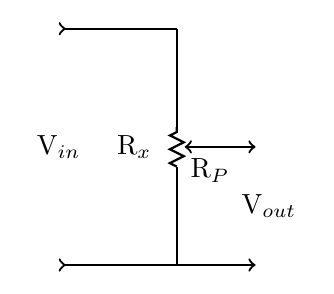
\begin{tikzpicture}[circuit ee IEC]
      \node at (0,1.5) {V$_{in}$}; % Vin label
      \draw[thick,>->] (0,0) -- (2.5,0); % Wiring 
      \draw[thick,>-] (0,3) -- (1.5,3); % Wiring
      \draw[thick](1.5,0) -- (1.5,1.25)(1.5,1.75) -- (1.5,3); % Wiring
      \draw[snake=zigzag,segment length=5,thick] (1.5,1.25) -- (1.5,1.75); % lower resistor
      \node[left] at (1.3,1.5){R$_{x}$}; % Rx label
      \node[right] at (1.55,1.2){R$_{P}$}; % RP label
      \draw[thick,<->] (1.6,1.5) -- (2.5,1.5); % Wiring
      \node[right] at (2.2,0.75) {V$_{out}$}; % Vout label
   \end{tikzpicture}
   \caption{Variable voltage divider}
   \label{fig:vdVariableVoltDiv}
\end{marginfigure}

The voltage divider in Figure \ref{fig:vdVoltDivIsolated} supplies a fixed voltage ratio. It is also possible for voltage dividers to supply a variable ratio. This is done with a device called a \textbf{potentiometer}. A potentiometer is a variable resistor whose resistance can be changed by turning a dial. Figure \ref{fig:vdVariableVoltDiv} shows a schematic of a potentiometer used as a variable voltage divider. The resistance of the entire potentiometer is R$_{x}$ and R$_{P}$ is the portion of this controlled by the dial. If the dial is adjusted so that R$_{p}$ is equal to R$_{x}$, then V$_{out}$ is equal to V$_{in}$. Likewise V$_{out}$ becomes zero if the dial is adjusted so that R$_{P}$ is zero.

Suppose two more resistors are added to the potentiometer to get the circuit shown in Figure \ref{fig:vdThreeResistVoltDiv}. The derivation for Equation \ref{equ:vdVout2} involves a loop with two resistors, but in fact can work for any number of resistors. The total series resistance would be on the bottom of the ratio. The output voltage V$_{out}$ could be taken across any or all of the resistors in the circuit and the value of these resistors would go on the top of the ratio. So, the output voltage will be

\begin{marginfigure}
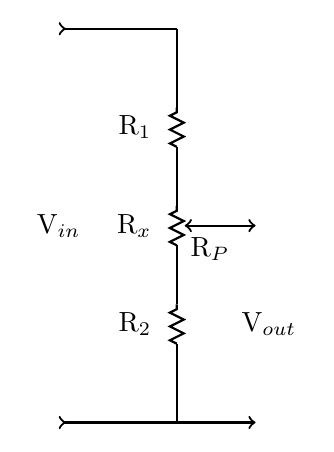
\begin{tikzpicture}
    \node at (0,2.5) {V$_{in}$}; % Vin label
    \draw[thick,>->] (0,0) -- (2.5,0); % Wiring 
    \draw[thick,>-] (0,5) -- (1.5,5); % Wiring
    \draw[thick](1.5,0) -- (1.5,1)(1.5,1.5) -- (1.5,2.25)(1.5,2.75)--(1.5,3.5)(1.5,4)--(1.5,5); % Wiring
    \draw[snake=zigzag,segment length=5,thick] (1.5,1) -- (1.5,1.5); % lower resistor
    \draw[snake=zigzag,segment length=5,thick] (1.5,2.25) -- (1.5,2.75); % middle resistor
    \draw[snake=zigzag,segment length=5,thick] (1.5,3.5) -- (1.5,4); % upper resistor
    \node[left] at (1.3,2.5){R$_{x}$}; % Rx label
    \node[right] at (1.55,2.2){R$_{P}$}; % RP label
    \node[left] at (1.3,3.75){R$_{1}$}; % R1 label
    \node[left] at (1.3,1.25){R$_{2}$}; % R2 label
    \draw[thick,<->] (1.6,2.5) -- (2.5,2.5); % Wiring
    \node[right] at (2.2,1.25) {V$_{out}$}; % Vout label
\end{tikzpicture}
\caption{Voltage divider with three resistors}
\label{fig:vdThreeResistVoltDiv}
\end{marginfigure}

\begin{equation}
V_{out}=V_{in}\frac{R_{P}+R_{2}}{R_{1}+R_{2}+R_{x}}.
\label{equ:vdVout3}
\end{equation}
This setup produces a range of voltages for V$_{out}$, which can be controlled by the dial on the potentiometer. The output voltage has a minimum greater than zero and a maximum less than V$_{in}$, as determined by R$_{1}$ and R$_{2}$.The minimum output voltage, V$_{min}$, occurs when R$_{P}$ is zero so

\begin{equation}
V_{min}=V_{in}\frac{R_{2}}{R_{1}+R_{2}+R_{x}},
\label{equ:vdVmin}
\end{equation}
and the maximum output voltage, Vmax, arises when RP equals Rx which gives

\begin{equation}
V_{max}=V_{in}\frac{R_{x}+R_{2}}{R_{1}+R_{2}+R_{x}}.
\label{equ:vdVmax}
\end{equation}

Not only do voltage dividers exist explicitly as the circuits shown in Figures \ref{fig:vdBasicVD}-\ref{fig:vdThreeResistVoltDiv}. They also exist implicitly whenever any two circuits are connected together. There is a division of voltage between the output of any circuit and the input of a second circuit. For example, imagine that a single resistor is connected to a power supply as shown in Figure \ref{fig:vdPowerSupply}. Here, the second circuit is composed of a single resistor R$_{L}$. Typically, R$_{L}$ is called the \textbf{load}, or in this case the \textbf{load resistor}.

\begin{marginfigure}
  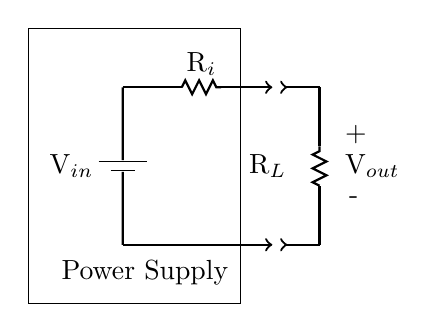
\begin{tikzpicture}[circuit ee IEC]
  \draw[thick] (0,2) to [battery] (0,0);
      \node at (-0.65,1) {V$_{in}$}; % Vin label
      \draw[snake=zigzag,segment length=5,thick] (0.75,2) -- (1.25,2); % upper resistor
      \draw[thick](0,2)--(0.75,2); % Wiring
      \draw[thick,->](1.25,2)--(1.9,2); %wiring
      \draw[thick,->] (0,0) -- (1.9,0); % Wiring
      \draw[thick,>-] (2,2) -- (2.5,2); % Wiring
      \draw[thick,>-] (2,0) -- (2.5,0); % Wiring
      \draw[thick](2.5,0)--(2.5,0.75)(2.5,1.25)--(2.5,2); % Wiring
      \draw[snake=zigzag,segment length=5,thick] (2.5,0.75) -- (2.5,1.25); % upper resistor
      \node[text centered] at (1,2.3){R$_{i}$}; % Ri label
      \node[left] at (2.2,1){R$_{L}$}; % RL label
      \node[right] at (2.7,1) {V$_{out}$}; % Vout label
      \node[right] at (2.7,1.4) {+}; % Vout + label
      \node[right] at (2.75,0.6) {-}; % Vout - label
      \node[right] at (-0.9,-0.35) {Power Supply}; % Power Supply label
      \draw  (-1.2,2.75) rectangle (1.5,-0.75); % Power Supply Box
\end{tikzpicture}
\caption{Power supply with internal resistor}
\label{fig:vdPowerSupply}
\end{marginfigure}

Ideally, it would be expected that the entire voltage, V$_{in}$, would be developed across the load resistor. However, what happens in practice is that the voltage across the load, V$_{out}$, is always somewhat smaller than V$_{in}$. Moreover, the smaller the value of R$_{L}$, the larger the discrepancy between V$_{out}$ and V$_{in}$. This situation can be neatly explained by the addition of an internal resistor, R$_{i}$. The voltage is now seen as being split between the load resistor R$_{L}$, and the internal resistance R$_{i}$. The basic voltage divider formula, Equation \ref{equ:vdVout2}, can be used to find V$_{out}$ as before to get

\begin{equation}
V_{out}=V_{in}\frac{R_{L}}{R_{L}+R_{i}}.
\label{equ:vdVout4}
\end{equation}

What is now observable is that the voltage across R$_{L}$ is less than the voltage being supplied by the power supply. If R$_{i}$ is much smaller than R$_{L}$, V$_{out}$ is, to a reasonable approximation, equal to V$_{in}$. At the same time, if the value of R$_{i}$ is close to the value of R$_{L}$, then V$_{out}$ will only be a portion of V$_{in}$. If R$_{i}$ were much larger than R$_{L}$ this effect would be dramatically increased and almost no voltage would be across R$_{L}$. For perfect power supplies R$_{i}$ is zero which means that V$_{out}$ = V$_{in}$ or any load resistor.

\begin{equation}
\frac{1}{V_{out}}=\frac{R_{i}}{V_{in}}\frac{1}{R_{L}}+\frac{1}{V_{in}}.
\label{equ:vdVout5}
\end{equation}

With Equation \ref{equ:vdVout5}, R$_{i}$ can be found by connecting a variable load and measuring V$_{out}$ across different load resistances. It can be seen that plotting $\frac{1}{V_{out}}$ versus $\frac{1}{R_{L}}$ yields a straight line with a slope of $\frac{R_{i}}{V_{in}}$ from which R$_{i}$ can be found.

So what is internal resistance exactly? Th\'{e}venin answered this by showing that from the point of view of any resistor in a circuit, the rest of the circuit is equivalent to a voltage source with a series internal resistance, just as in Figure \ref{equ:vdVmin}. For example, the left side of Figure \ref{fig:vdTheveninEqu} shows a circuit containing a number of voltage sources and resistors. From the point of view of a single resistor such as R$_{5}$, the entire remaining part of the original circuit is equivalent to a single voltage source in series with a single resistor, as shown on the right side of Figure \ref{fig:vdTheveninEqu}. This is called the Th\'{e}venin equivalent circuit. The voltage source, V$_{th}$, is called the Th\'{e}venin equivalent voltage and the resistor, R$_{th}$, is called the Th\'{e}venin equivalent resistance. Comparing this with Figure  \ref{fig:vdPowerSupply}, it is seen that the Th\'{e}venin equivalent circuit is a power supply with an internal resistance driving a load consisting of the chosen component, in this case R$_{5}$.

\begin{figure}
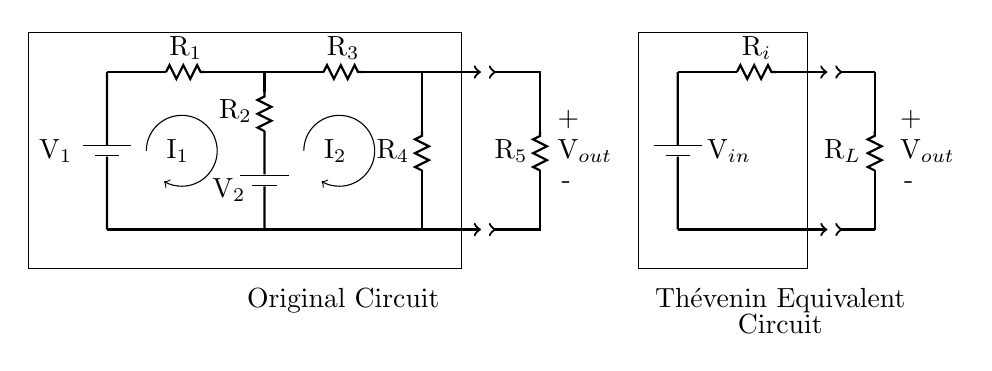
\begin{tikzpicture}[circuit ee IEC]

%%% Diagram on left of page

\draw[thick] (0,2) to [battery] (0,0); % V1
\node at (-0.65,1) {V$_{1}$}; % V1 label
\draw[thick] (2,1.25) to [battery] (2,0); % V2
\node at (1.55,0.5) {V$_{2}$}; % V2 label
\draw[snake=zigzag,segment length=5,thick] (0.75,2) -- (1.25,2); % R1
\node[text centered] at (1,2.3){R$_{1}$}; % R1 label
\draw[snake=zigzag,segment length=5,thick] (2,1.25) -- (2,1.75); % R2
\node[right] at (1.3,1.5){R$_{2}$}; % R2 label
\draw[snake=zigzag,segment length=5,thick] (2.75,2) -- (3.25,2); % R3
\node[text centered] at (3,2.3){R$_{3}$}; % R3 label
\draw[snake=zigzag,segment length=5,thick] (4,0.75) -- (4,1.25); % R4
\node[right] at (3.3,1){R$_{4}$}; % R4 label
\draw[snake=zigzag,segment length=5,thick] (5.5,0.75) -- (5.5,1.25); % R5
\node[right] at (4.8,1){R$_{5}$}; % R5 label
\draw[thick](0,2)--(0.75,2); % Wiring
\node[right] at (5.6,1) {V$_{out}$}; % Vout label
\node[right] at (5.6,1.4) {+}; % Vout + label
\node[right] at (5.65,0.6) {-}; % Vout - label
\draw[->,] (0.5,1) arc (180:-120:0.45); % left loop current direction arrow
\node[text centered] at (0.9,1){I$_{1}$}; % I1 label
\draw[->] (2.5,1) arc (180:-120:0.45); % middle loop current direction arrow
\node[text centered] at (2.9,1){I$_{2}$}; % I2 label
\draw[thick](1.25,2)--(2.75,2)(2,1.75)--(2,2)(4,0)--(4,0.75)(4,1.25)--(4,2); % wiring
\draw[thick,->] (3.25,2) -- (4.75,2); % Wiring
\draw[thick,>-] (4.85,2)--(5.5,2) -- (5.5,1.25); % Wiring
\draw[thick,->] (0,0)--(4.75,0); % Wiring
\draw[thick,>-] (4.85,0)--(5.5,0)--(5.5,0.75); % Wiring
\node[text centered] at (3,-0.9) {Original Circuit}; % Original Circuit label
\draw  (-1,2.5) rectangle (4.5,-0.5); % Original Circuit Box

% Diagram on right side of page

 \draw[thick] (7.25,2) to [battery] (7.25,0);
      \node at (7.9,1) {V$_{in}$}; % Vin label
      \draw[snake=zigzag,segment length=5,thick] (8,2) -- (8.5,2); % upper resistor
      \draw[thick](7.25,2)--(8,2); % Wiring
      \draw[thick,->](8.5,2)--(9.15,2); %wiring
      \draw[thick,->] (7.25,0) -- (9.15,0); % Wiring
      \draw[thick,>-] (9.25,2) -- (9.75,2); % Wiring
      \draw[thick,>-] (9.25,0) -- (9.75,0); % Wiring
      \draw[thick](9.75,0)--(9.75,0.75)(9.75,1.25)--(9.75,2); % Wiring
      \draw[snake=zigzag,segment length=5,thick] (9.75,0.75) -- (9.75,1.25); % upper resistor
      \node[text centered] at (8.25,2.3){R$_{i}$}; % Ri label
      \node[left] at (9.7,1){R$_{L}$}; % RL label
      \node[right] at (9.95,1) {V$_{out}$}; % Vout label
      \node[right] at (9.95,1.4) {+}; % Vout + label
      \node[right] at (10,0.6) {-}; % Vout - label
      \node[text centered] at (8.55,-0.9) {Th\'{e}venin Equivalent}; % Thevenin Equivalent label
      \node[text centered] at (8.55,-1.2) {Circuit}; % Thevenin Equivalent label
      \draw (6.75,2.5) rectangle (8.9,-0.5); % Thevenin Equivalent Box
\end{tikzpicture}
\caption{Th\'{e}venin equivalent circuit}
\label{fig:vdTheveninEqu}
\end{figure}

There is a standard procedure for calculating V$_{th}$ and R$_{th}$. The Th�venin equivalent voltage is equal to the voltage that would be found across the terminals without anything attached to it. Here, R$_{5}$ is the reference component so it is replaced with an open circuit. So the voltage across R$_{4}$ is the voltage being output by this circuit and is equal to V$_{th}$. In this example the Th�venin voltage is equal to the product of the current in the second loop, I$_{2}$, and the resistance R$_{4}$. If the value for all the voltage sources and resistors are known, the current across R$_{4}$ can be found by solving for the loop currents. This will yield the Th�venin voltage as being

\begin{equation}
V_{th}=I_{2}R_{4}.
\label{equ:vdVth}
\end{equation}

To find R$_{th}$, R$_{5}$ is again removed and all voltage sources in the circuit are replaced with their internal resistance. In this case the voltage sources are assumed to be ideal and are replaced with short circuits. The Th\'{e}venin resistance is then the equivalent resistance at the open terminals. For the circuit in Figure \ref{fig:vdTheveninEqu} this is

\begin{equation}
R_{th}=\left(\left(R_{1}\parallel R_{2}\right)+R_{3}\right)\parallel R_{4},
\label{equ:vdRth}
\end{equation}
where $\parallel$ indicates that the resistors are to be added in parallel.

Another way to measure V$_{th}$ and R$_{th}$ is by knowing that the Th�venin equivalent circuit in Figure \ref{fig:vdTheveninEqu} is identical to the circuit depicted in Figure \ref{fig:vdPowerSupply}. Equation \ref{equ:vdVout5} can therefore be used to find V$_{th}$ and R$_{th}$ by varying R$_{5}$. Here, V$_{out}$ is the voltage across R$_{5}$, and V$_{in}$ and R$_{i}$ are V$_{th}$ and R$_{th}$ respectively. Again, plotting $\frac{1}{V_{out}}$ versus $\frac{1}{R_{5}}$ should yield a straight line. This method produces a graph giving R$_{th}$ and V$_{th}$ from the slope and intercept.

So by attaching a load resistor to a circuit, in the case of Figure \ref{fig:vdTheveninEqu} this was R$_{5}$, the voltage across the resistor is dependent on the internal resistance as explained by the voltage divider rule. The effect that a load resistor has on circuits is called circuit loading.  Imagine the basic voltage divider in Figure \ref{fig:vdVoltDivIsolated} where a voltmeter is used to measure V$_{out}$. Just like the power supply, voltmeters have some internal resistance. In the analysis of Equation \ref{equ:vdVout2}, it was assumed that no current goes into the voltmeter, which is true only for an ideal voltmeter. 

The effect that non ideal voltmeters have on voltage dividers is shown in Figure \ref{fig:vdVoltMeterInternalR}. This schematic is similar to Figure \ref{fig:vdVoltDivConnect} with the exception that the voltmeter now has an internal resistance R$_{i}$. Ideally, the voltage across R$_{2}$ is the ratio of R$_{2}$ to the entire resistance, R$_{1}$ + R$_{2}$. Once a voltmeter is connected, the voltage is split between R$_{1}$ and the combined resistance of R$_{2}$ and R$_{i}$, in parallel. In Figure \ref{fig:vdVoltMeterInternalR}, V$_{r}$ is the voltage read by the voltmeter and V$_{out}$, although not explicitly shown, is the actual voltage across R$_{2}$ without the voltmeter attached.This equivalent resistance is given by

\begin{figure}
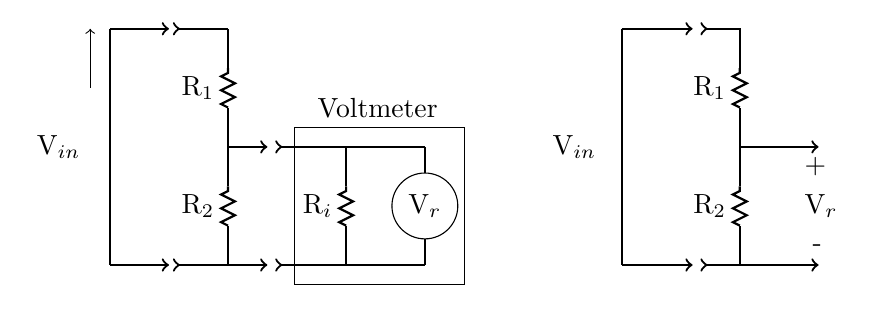
\begin{tikzpicture}
      \draw[thick] (0,3) to [battery] (0,0); % battery
      \node at (-0.65,1.5) {V$_{in}$}; % Vin label
       \draw[thick,->] (0,0) -- (0.75,0); % Wiring 
      \draw[thick,>->] (0.8,0) -- (2,0); % Wiring
      \draw[thick,->] (0,3) -- (0.75,3); % Wiring
      \draw[thick,>-] (0.8,3) -- (1.5,3); % Wiring
      \draw[thick](1.5,0) -- (1.5,0.5)(1.5,1) -- (1.5,2)(1.5,2.5) -- (1.5,3); % Wiring
      \draw[snake=zigzag,segment length=5,thick] (1.5,2) -- (1.5,2.5); % R1
      \node[left] at (1.45,2.25){R$_{1}$}; % R1 label
      \draw[snake=zigzag,segment length=5,thick] (3,0.5) -- (3,1); % Ri
      \node[left] at (2.95,0.75){R$_{i}$}; % Ri label
      \draw[snake=zigzag,segment length=5,thick] (1.5,0.5) -- (1.5,1); % R2
      \node[left] at (1.45,0.75){R$_{2}$}; % R2 label
      \draw[thick] (4,1.5) -- (4,0); % voltmeter wires
      \draw[thick,->] (1.5,1.5) -- (2,1.5); % Wiring
      \draw[thick,>-] (2.1,1.5) -- (4,1.5); % Wiring
      \draw[thick,>-] (2.1,0) -- (4,0); % Wiring
      \draw[thick](3,0)--(3,0.5)(3,1)--(3,1.5); %Wiring
      \node[black,fill=white,draw=black,shape=circle,scale=1] at (4,0.75) {V$_{r}$}; % voltmeter   
	  \draw (2.35,1.75) rectangle (4.5,-0.25);
      \node[text centered] at (3.4,2) {Voltmeter};
      \draw[->](-0.25,2.25) -- (-0.25,3); % current arrow


%%% Diagram on right side of page
      
      \draw[thick] (6.5,3) to [battery] (6.5,0); % battery
      \node at (5.9,1.5) {V$_{in}$}; % Vin label
      \draw[snake=zigzag,segment length=5,thick] (8,2) -- (8,2.5); % upper resistor
      \node[left] at (7.95,2.25){R$_{1}$}; % R1 label
      \draw[snake=zigzag,segment length=5,thick] (8,0.5) -- (8,1); % lower resistor
      \node[left] at (7.95,0.75){R$_{2}$}; % R2 label
      \node[right] at (8.7,0.75) {V$_{r}$}; % Vr label
      \node[right] at (8.7,1.25) {+}; % Vout + label
      \node[right] at (8.8,0.25) {-}; % Vout - label
      \draw[thick,->] (8,1.5) -- (9,1.5); % Wiring
      \draw[thick,->](6.5,0)--(7.4,0);  % Wiring
      \draw[thick,->](6.5,3)--(7.4,3);  % Wiring
      \draw[thick,->](8,0)--(9,0);  % Wiring
      \draw[thick,>-] (7.5,0) -- (8,0) -- (8,0.5); % Wiring
      \draw[thick,>-] (7.5,3) -- (8,3)-- (8,2.5); % Wiring
      \draw[thick](8,1)--(8,2); % Wiring
\end{tikzpicture}
\caption{Internal Resistance of Voltmeter}
\label{fig:vdVoltMeterInternalR}
\end{figure}


\begin{equation}
R_{eq}=R_{2}\parallel R_{i}=\frac{R_{2}R_{i}}{R_{2}+R_{i}}.
\label{equ:vdReq}
\end{equation}

It is seen that if R$_{i}$ is much larger than R$_{2}$, then R$_{eq}$ is nearly equal to R$_{2}$, and Equation \ref{equ:vdVout2} still holds. This is what would be expected from an ideal voltmeter. If this is not the case then R$_{eq}$ will be smaller than R$_{2}$. So a larger portion of voltage will develop across R$_{1}$ than before the voltmeter was connected. The voltage measured by the voltmeter will now be smaller than expected. This effect is called meter loading and is seen when R$_{2}$ in Equation \ref{equ:vdVout2} is replaced with R$_{eq}$ to get

\begin{equation}
V_{r}=V_{in}\frac{R_{eq}}{R_{eq}+R_{1}}\neq V_{out}.
\label{equ:vdVr}
\end{equation}

Equation \ref{equ:vdVr} gives the output voltage, taking the effect of the voltmeter on the circuit into account. It can be used to calculate the internal resistance of the voltmeter. Furthermore, it is possible to rearrange Equation \ref{equ:vdVr} to find the voltmeter internal resistance by

\begin{equation}
R_{i}=\frac{R_{1}R_{2}}{R_{2}\left(\frac{V_{in}}{V_{r}}-1\right)-R_{1}},
\label{equ:vdRi}
\end{equation}
if R$_{1}$, R$_{2}$ and V$_{in}$ are known, and V$_{r}$ is the reading from the voltmeter.

It has been shown that voltage dividers occur in many circuits containing resistors and/or devices in series. In this experiment several different voltage dividers are examined. A simple voltage divider similar to the one seen in Figure \ref{fig:vdBasicVD} is constructed to examine the voltage divider formula. A potentiometer can then be inserted to check Equations \ref{equ:vdVout3}-\ref{equ:vdVmax}. The power supply can then be probed to find its internal resistance and see the effects of having a power supply with a large internal resistance. Th�venin equivalence can be tested using the three methods previously described, calculation of theoretical values for V$_{th}$ and R$_{th}$, taking direct measurements, and the use of a variable load resistor.

Two multimeters are used in this experiment, the Philips digital meter and the Sanwa analog meter. The Philips multimeter is close to ideal in many situations and is used for most of the measurements in this experiment. The Sanwa multimeter, which is farther from ideal, is used to see the effects of meter loading. The Philips multimeter also has the necessary precision required for observing the small internal resistance of the power supply. 

In this experiment the Philips multimeter is used for taking voltage and resistance measurements. All connections are made to the red V Jack and the black COM jack. Switching between voltage and resistance readings is done via buttons along the bottom of the multimeter, under the display. The DC voltage function is selected by the V\raisebox{0.3 em}{\Beam} button and the resistance function is chosen with the 2W button. For some measurements it may be necessary to change the range of the meter. The three top right buttons on the instrument are the ranging controls. The range can be changed to automatic or manual with the AUT/MAN button. In manual mode the UP and DOWN buttons are used to change the range. Auto ranging is recommended unless otherwise specified in the procedure. When measuring resistance, be sure to disconnect any power supplies from the circuit. The internal resistance of the Philips voltmeter is 10 M$\Omega$.

The Sanwa multimeter is an analog meter with a fairly low input resistance. This multimeter will be used to witness the effect of voltmeter loading. For this experiment the multimeter is in a box and all connections are done using the terminals on the outside of this box. The range can be set using the dial on the front of the device. Useful ranges for this experiment are 0.5 V, 2.5 V, 10 V and 50 V. The internal resistance of the Sanwa multimeter is directly proportional to the voltage range it is reading in and is 20 k$\Omega$/V. For example the internal resistance at the 10 V setting should be 10 V x 20 k$\Omega$/V, which is 200 k$\Omega$.



\section{Experimental Procedure}
\begin{enumerate}

\begin{marginfigure}
      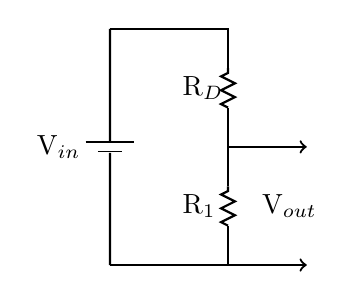
\begin{tikzpicture}[circuit ee IEC]
      \draw[thick] (0,3) to [battery] (0,0); % battery
      \node at (-0.65,1.5) {V$_{in}$}; % Vin label
      \draw[thick] (0,0) -- (1.5,0) -- (1.5,0.5)(1.5,1) -- (1.5,2)(1.5,2.5) -- (1.5,3) -- (0,3);  %wiring
      \draw[snake=zigzag,segment length=5,thick] (1.5,2) -- (1.5,2.5); % upper resistor
	  \node[right] at (0.8,2.25){R$_{D}$}; % RD label
      \draw[snake=zigzag,segment length=5,thick] (1.5,0.5) -- (1.5,1); % lower resistor
      \node[right] at (0.8,0.75){R$_{1}$}; % R1 label
      \draw[thick,->] (1.5,0) -- (2.5,0); % wiring
      \draw[thick,->] (1.5,1.5) -- (2.5,1.5); % wiring
      %\node[black,fill=white,draw=black,shape=circle,scale=1] at (2.5,0.75) {V_{out}}; % voltmeter
      \node[left] at (2.75,0.75) {V$_{out}$}; % Vout label
\end{tikzpicture}
\caption{Step 1 Basic voltage divider}
\label{fig:vdBasicVD2}
\end{marginfigure}

\item Construct the basic voltage divider depicted in Figure \ref{fig:vdBasicVD2} with R$_{D}$ = 100 $\Omega$ and R$_{1}$ = 20 $\Omega$ . With the power supply disconnected, measure the resistance of R$_{D}$ and R$_{1}$ directly with the Philips multimeter. Turn on the power supply and connect the Philips multimeter across R$_{1}$ and take measurements of V$_{out}$ while changing V$_{in}$ from 1 V to 5 V. Take a minimum of 9 data points.

\begin{marginfigure}
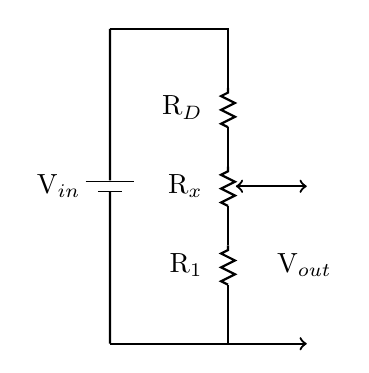
\begin{tikzpicture}[circuit ee IEC]
    \draw[thick] (0,4) to [battery] (0,0); % battery
    \node at (-0.65,2) {V$_{in}$}; % Vin label
    \draw[thick] (0,4) -- (1.5,4) -- (1.5,3.25); % Wiring
    \draw[thick](1.5,0) -- (1.5,0.75)(1.5,1.25) -- (1.5,1.75)(1.5,2.25)--(1.5,2.75); % Wiring
    \draw[thick,->](0,0) -- (2.5,0); % Wiring
    \draw[thick,<->] (1.6,2) -- (2.5,2); % Wiring
    \draw[snake=zigzag,segment length=5,thick] (1.5,0.75) -- (1.5,1.25); % lower resistor
    \draw[snake=zigzag,segment length=5,thick] (1.5,1.75) -- (1.5,2.25); % middle resistor
    \draw[snake=zigzag,segment length=5,thick] (1.5,2.75) -- (1.5,3.25); % upper resistor
    \node[left] at (1.3,2){R$_{x}$}; % Rx label
    \node[left] at (1.3,3){R$_{D}$}; % RD label
    \node[left] at (1.3,1){R$_{1}$}; % R1 label
    \node[right] at (2,1) {V$_{out}$}; % Vout label
\end{tikzpicture}
\caption{Voltage divider with three resistors}
\label{fig:vdThreeResistVoltDiv2}
\end{marginfigure}

\item Measure the resistance of the potentiometer, R$_{x}$, using the Ohmmeter across the red and black terminals. Build the circuit in Figure \ref{fig:vdThreeResistVoltDiv2} with R$_{D}$ = 100 $\Omega$ and R$_{1}$ = 20 $\Omega$. This circuit has a V$_{min}$ and V$_{max}$ which can be found experimentally. Set V$_{in}$ to approximately 1 V and measure V$_{in}$ with the Phillips multimeter. Disconnect the Phillips multimeter from the power supply and use it to take measurements of V$_{out}$ for dial readings 1-10 on the potentiometer. 

\item Connect R$_{D}$ = 100 $\Omega$ to the positive output terminal of the power supply. This will show the effects of having a power supply with a high output resistance. Connect a resistance decade box in series to serve as a variable load. The setup should resemble Figure \ref{fig:vdPowerSupply}. Because the 100 $\Omega$ resistor is much larger than the actual internal resistance of the power supply, R$_{i}$ is essentially equal to the value of R$_{D}$. Set the power supply to 1 V. Using the Philips multimeter, take at least 10 measurements of V$_{out}$ while varying the load resistance from 10 $\Omega$  to 10 k$\Omega$.

\item Remove R$_{D}$ from the circuit in step 3. Now, R$_{i}$ is the actual internal resistance of the power supply to be measured. Again set the power supply to 1 V and take measurements, with the Philips multimeter, of V$_{out}$ for load resistance's ranging from  1 $\Omega$  to 10 $\Omega$.

\item Choose one of the circuits in Figures \ref{fig:vdOptA}-\ref{fig:vdOptC} and build it. The Th\'{e}venin equivalent voltage and resistance can be found by direct measurements and by calculation. Set the power supply between 1 V and 5 V. Measure V$_{th}$ directly with a voltmeter. Replace the power supply with a short and measure R$_{th}$ directly with an ohmmeter. Remember to disconnect the power from a circuit before taking measurements of resistance with an ohmmeter.


\begin{marginfigure}
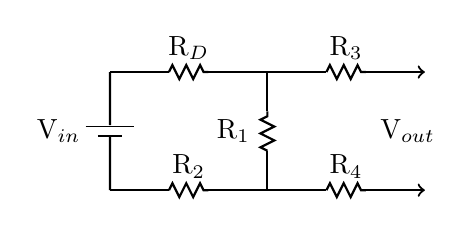
\begin{tikzpicture}[circuit ee IEC]
\draw[thick] (0,1.5) to [battery] (0,0); % battery
\node at (-0.65,0.75) {V$_{in}$}; % Vin label
\draw[snake=zigzag,segment length=5,thick] (2,0.5) -- (2,1); % R1
\node[left] at (1.9,0.75){R$_{1}$}; % R1 label
\draw[snake=zigzag,segment length=5,thick] (0.75,1.5) -- (1.25,1.5); % RD
\node[text centered] at (1,1.8){R$_{D}$}; % RD label
\draw[snake=zigzag,segment length=5,thick] (0.75,0) -- (1.25,0); % R2
\node[text centered] at (1,0.3){R$_{2}$}; % R2 label
\draw[snake=zigzag,segment length=5,thick] (2.75,1.50) -- (3.25,1.5); % R3
\node[text centered] at (3,1.8){R$_{3}$}; % R3 label
\draw[snake=zigzag,segment length=5,thick] (2.75,0) -- (3.25,0); % R4
\node[text centered] at (3,0.3){R$_{4}$}; % R4 label
\node[left] at (4.25,0.75) {V$_{out}$}; % Vout label
\draw[thick](0,1.5)--(0.75,1.5)(1.25,1.5)--(2.75,1.5)(2,1.5)--(2,1) ;% Wiring
\draw[thick](0,0)--(0.75,0)(1.25,0)--(2.75,0)(2,0)--(2,0.5);% Wiring
\draw[thick,->](3.25,1.5)--(4,1.5); % Wiring
\draw[thick,->](3.25,0)--(4,0); % Wiring
\end{tikzpicture}
\caption{Step 5 Optional circuit diagram A}
\label{fig:vdOptA}
\end{marginfigure}

\begin{marginfigure}
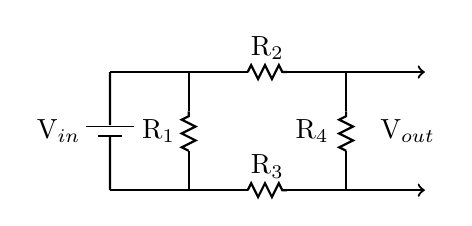
\begin{tikzpicture}[circuit ee IEC]
\draw[thick] (0,1.5) to [battery] (0,0); % battery
\node at (-0.65,0.75) {V$_{in}$}; % Vin label
\draw[snake=zigzag,segment length=5,thick] (1,0.5) -- (1,1); % R1
\node[left] at (0.95,0.75){R$_{1}$}; % R1 label
\draw[snake=zigzag,segment length=5,thick] (1.75,1.5) -- (2.25,1.5); % R2
\node[text centered] at (2,1.8){R$_{2}$}; % R2 label
\draw[snake=zigzag,segment length=5,thick] (1.75,0) -- (2.25,0); % R3
\node[text centered] at (2,0.3){R$_{3}$}; % R3 label
\draw[snake=zigzag,segment length=5,thick] (3,0.5) -- (3,1); % R4
\node[left] at (2.9,0.75){R$_{4}$}; % R4 label
\node[left] at (4.25,0.75) {V$_{out}$}; % Vout label
\draw[thick](0,1.5)--(1.75,1.5)(1,1.5)--(1,1)(3,1.5)--(3,1) ;% Wiring
\draw[thick](0,0)--(1.75,0)(1,0)--(1,0.5)(3,0)--(3,0.5) ;% Wiring
\draw[thick,->](2.25,1.5)--(4,1.5); % Wiring
\draw[thick,->](2.25,0)--(4,0); % Wiring
\end{tikzpicture}
\caption{Step 5 Optional circuit diagram B}
\label{fig:vdOptB}
\end{marginfigure}

\begin{marginfigure}
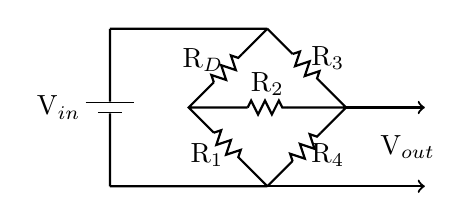
\begin{tikzpicture}[circuit ee IEC]
\draw[thick] (0,2) to [battery] (0,0); % battery
\node at (-0.65,1) {V$_{in}$}; % Vin label
\draw[snake=zigzag,segment length=5,thick] (1.32,0.68) -- (1.68,0.32); % R1
\node[right] at (0.9,0.4){R$_{1}$}; % R1 label
\draw[snake=zigzag,segment length=5,thick] (1.75,1) -- (2.25,1); % R2
\node[text centered] at (2,1.3){R$_{2}$}; % R2 label
\draw[snake=zigzag,segment length=5,thick] (1.32,1.32) -- (1.68,1.68); % RD
\node[right] at (0.8,1.6){R$_{D}$}; % RD label
\draw[snake=zigzag,segment length=5,thick] (2.32,1.68) -- (2.68,1.32); % R3
\node[left] at (3.1,1.63){R$_{3}$}; % R3 label
\draw[snake=zigzag,segment length=5,thick] (2.32,0.32) -- (2.68,0.68); % R4
\node[left] at (3.1,0.4){R$_{4}$}; % R4 label
\node[left] at (4.25,0.5) {V$_{out}$}; % Vout label
\draw[thick](0,2)--(2,2)(2,2)--(1.68,1.68)(2,2)--(2.32,1.68) ;% Wiring
\draw[thick](0,0)--(2,0)(2,0)--(1.68,0.32)(2,0)--(2.32,0.32) ;% Wiring
\draw[thick](1.32,1.32)--(1,1)--(1.32,0.68)(1,1)--(1.75,1); % Wiring
\draw[thick](2.68,1.32)--(3,1)--(2.68,0.68)(3,1)--(2.25,1);
\draw[thick,->](3,1)--(4,1); % Wiring
\draw[thick,->](2,0)--(4,0); % Wiring
\end{tikzpicture}
\caption{Step 5 Optional circuit diagram C}
\label{fig:vdOptC}
\end{marginfigure}


\begin{marginfigure}
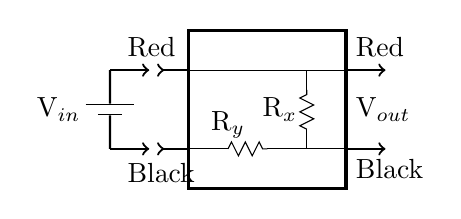
\begin{tikzpicture}[circuit ee IEC]
\draw[thick] (0,1.5) to [battery] (0,0.5); % battery
\node at (-0.65,1) {V$_{in}$}; % Vin label
\draw[very thick](1,2) rectangle (3,0);
\draw[snake=zigzag,segment length=5] (1.5,0.5) -- (2,0.5); % Ry
\node[text centered] at (1.5,0.8){R$_{y}$}; % Ry label
\draw[snake=zigzag,segment length=5] (2.5,0.75) -- (2.5,1.25); % Rx
\node[left] at (2.5,1){R$_{x}$}; % Rx label
\node[right] at (3,1) {V$_{out}$}; % Vout label
\draw(1,0.5)--(1.5,0.5)(2,0.5)--(3,0.5)(2.5,0.5)--(2.5,0.75) ;% Wiring
\draw(1,1.5)--(3,1.5)(2.5,1.5)--(2.5,1.25);% Wiring
\draw[thick,->](0,0.5)--(0.5,0.5); % Wiring
\draw[thick,->](0,1.5)--(0.5,1.5); % Wiring
\draw[thick,->](3,0.5)--(3.5,0.5); % Wiring
\draw[thick,->](3,1.5)--(3.5,1.5); % Wiring
\draw[thick,>-](0.6,1.5)--(1,1.5); % Wiring
\draw[thick,>-](0.6,0.5)--(1,0.5); % Wiring
\node[right] at (0.1,1.8) {Red}; % Red label left
\node[right] at (0.1,0.2) {Black}; % Black label right
\node[right] at (3,1.8) {Red}; % Red label left
\node[right] at (3,0.25) {Black}; % Black label right
\end{tikzpicture}
\caption{Voltage divider black box}
\label{fig:vdBlackBox}
\end{marginfigure}


\item Next, use an indirect approach to find the Th\'{e}venin equivalent voltage and resistance. Connect a resistance decade box across Vout for the circuit chosen in step 5. This is the load resistor R$_{L}$ and creates a voltage divider between R$_{th}$ and R$_{L}$. Take at least 10 measurements of V$_{out}$ across the load resistor, as the resistance is varied from 10 $\Omega$  to 10 k$\Omega$. Equation \ref{equ:vdVout5} can then be used to deduce the Th�venin equivalent voltage and resistance.
\item Similar to Figure \ref{fig:vdVoltDivIsolated}, a black box containing a voltage divider is provided as seen in Figure \ref{fig:vdBlackBox}. Using resistance measurements only, deduce the contents of the box.
\item Using the same black box as step 7, connect the positive end of the power supply to the red terminal of the black box, and the negative end to the black terminal. Set V$_{in}$ to 3 V and take voltage readings across the red and white terminals. Call this voltage V$_{r}$. Measure V$_{r}$ with the Philips multimeter at voltage ranges 3, 30 and 300.
\item Measure V$_{r}$ with the Sanwa analog meter at voltage ranges 0.5, 2.5, 10 and 50.
\end{enumerate}

\section{Error Analysis}

The wires used are assumed to be ideal, but they do have a small amount of resistance. For some steps such as finding the internal resistance of the power supply, the resistance in the wires may affect the value obtained. Another source of uncertainty arises from the self heating of the resistors when current passes through them. Also for a 5 digit multimeter like the Philips instrument, external noise can be seen in the variance of the lower digits. In this case, the error can be estimated as half the smallest non-varying digit. The uncertainties for voltage and resistance measurements for the multimeter are given in Tables \ref{tab:volunc} and \ref{tab:resunc}, respectively. The Sanwa multimeter accuracy is given by half the resolution of the scale for that range.

\begin{table}
\caption{The accuracy of the voltage measurements for the Philips multimeter.}
\centering
\begin{tabular}{|c|c|c|}
   \hline
     Range&$\%$ of reading&$\%$ of reading \\
     \hline
        \hline
     300 mV& 0.0025&0.0013\\
     3 V& 0.0020&0.0010\\
     30 V& 0.0025&0.0013\\
     300 V& 0.0025&0.0010\\
        \hline
\end{tabular}
\label{tab:volunc}
\end{table}

\begin{table}
\caption{The accuracy of the resistance measurements for the Philips multimeter.}
\centering
\begin{tabular}{|c|c|c|}
   \hline
     Range&$\%$ of reading&$\%$ of reading \\
     \hline
        \hline
     3 k$\Omega$& 0.01&0.0033\\
     300 k$\Omega$& 0.01&0.0033\\
    3 M$\Omega$& 0.02&0.0033\\
        \hline
\end{tabular}
\label{tab:resunc}
\end{table}
%For the Philips multimeter the basic uncertainty of each measurement is dependent on the range it is set to. The accuracy is given in $\pm$(\% of reading + \% of range). At range settings of 300 mV and 30 V the accuracy is 0.0025\% + 0.0013\%, for the 3 V range it is 0.0020\% + 0.0010\%, and for the 300 V range the accuracy is 0.0025\% + 0.0010\%. The accuracy of resistance measurements in the 3 k$\Omega$ and 300 k$\Omega$ range is 0.01\% + 0.0033\%. For the 3 M$\Omega$ range it is 0.02\% + 0.0033\%. 

\vspace{12pt}

\textbf{To be handed in to the laboratory instructor}

%%% begin prelab %%%
\section{Prelab}
\begin{enumerate}
\item Design a fixed voltage divider for a V$_{in}$ of 9 V and a V$_{out}$ of 1 V with a total resistance (R1+R2) of 1 M$\Omega$.
\item Design a variable voltage divider for a V$_{in}$ of 12 V, with an output ranging from 1 V to 4 V.
\item Suppose a power supply outputs 10.0 V with no load and the output drops to 9.8 V with a 1 k$\Omega$ load. What is the internal resistance of the power supply.
\item Calculate the Th�venin equivalent circuit for one of the three circuits in Figures \ref{fig:vdOptA}-\ref{fig:vdOptC}. Assume that R$_{D}$ = 100 $\Omega$, R$_{1}$ = 20.0 $\Omega$, R$_{2}$ = 27.0 $\Omega$, R$_{3}$ = 47.0 $\Omega$, R$_{4}$ = 100 $\Omega$ and V$_{in}$ = 3.0 V.
\item Using Figure \ref{fig:vdVoltMeterInternalR}, suppose R$_{1}$ = 110 k$\Omega$, R$_{2}$ = 330 k$\Omega$ and V$_{in}$ is 1 V. For this voltage divider calculate V$_{out}$. What will a voltmeter with 100 k$\Omega$ internal resistance measure for V$_{out}$.
\end{enumerate}
%%% end prelab %%%
\section{Data Requirements}
% continue numbering
\begin{enumerate}[resume]
\item A table containing V$_{out}$ and V$_{in}$ for the basic voltage divider and values of R$_{D}$ and R$_{1}$ as measured with the ohmmeter. Include all associated uncertainties.
\item A graph of V$_{out}$ versus V$_{in}$ for the basic voltage divider, including error bars.
\item The measured value of the potentiometer, R$_{x}$, as well as a table with V$_{out}$ and the dial reading numbers from step 2 of the \textbf{Experimental Procedure}. Include all relevant uncertainties.
\item A graph of V$_{out}$ versus dial reading and values of V$_{min}$ and V$_{max}$ for the variable divider.
\item A table with Vout, R$_{L}$, $\frac{1}{V_{out}}$, and $\frac{1}{R_{L}}$ from step 3 of the \textbf{Experimental Procedure}. Include uncertainties and the value of V$_{in}$.
\item A graph of  $\frac{1}{V_{out}}$ versus $\frac{1}{R_{L}}$ including error bars. Present measured and calculated values of R$_{D}$.
\item A table with V$_{out}$, R$_{L}$, $\frac{1}{V_{out}}$ and $\frac{1}{R_{L}}$ from step 4 of the \textbf{Experimental Procedure}. Include uncertainties and the value of V$_{in}$.
\item A graph of $\frac{1}{V_{out}}$ versus $\frac{1}{R_{L}}$ including error bars. Show the derived value for the internal resistance of the power supply, R$_{i}$.
\item Direct measurements of R$_{th}$ and V$_{th}$ from step 5.
\item A table with V$_{out}$, R$_{L}$, $\frac{1}{V_{out}}$ and $\frac{1}{R_{L}}$ from step 6. Include uncertainties and the value of V$_{in}$.
\item A graph of $\frac{1}{V_{out}}$ versus $\frac{1}{R_{L}}$ and values of V$_{th}$ and R$_{th}$ obtained from the slope and intercept.
\item Measured values of R$_{x}$ and R$_{y}$ in the black box from step 7 of the \textbf{Experimental Procedure}.
\item Values for V$_{r}$ from step 8 of the \textbf{Experimental Procedure} and the internal resistance of the Philips voltmeter at each range.
\item Values for V$_{r}$ from step 9 of the \textbf{Experimental Procedure} and the internal resistance of the Sanwa voltmeter at each range.
\end{enumerate}

\section{Discussion}
\begin{enumerate}[resume]
\item Based on the graph from the basic voltage divider, compare the ratio obtained from the graph to the calculated ratio.
\item Compare the behaviour of the variable voltage divider with the theoretically predicted performance.
\item For parts 3 and 4, compare the output voltage behaviour under varying loads for the high and low internal resistance power supplies. Why is a small internal resistance preferred for a power supply? What is the internal resistance of an ideal power supply?
\item For the circuit chosen in parts 5 and 6, compare the calculated, directly measured, and indirectly measured values of V$_{th}$ and R$_{th}$ of the Th\'{e}venin equivalent circuit.
\item Using the Measured values for R$_{x}$ and R$_{y}$, compare the voltmeter readings taken with the Philips and Sanwa multimeter to the expected value. Which multimeter is better for taking voltage measurements and why? What is the internal resistance of an ideal voltmeter?
\end{enumerate}

\AtEndDocument{\clearpage\ifodd\value{page}\else\null\clearpage\fi} % forces even page count, for double siding

\end{document}
